\documentclass[10pt,a4paper]{article}
\usepackage[utf8]{inputenc}
\usepackage[T1]{fontenc}
\usepackage{lmodern}
\usepackage[a4paper, margin=0.65in]{geometry}
\usepackage{amsmath, amssymb}
\usepackage{booktabs}
\usepackage{tabularx}
\usepackage{graphicx}
\usepackage{xcolor}
\usepackage{subcaption}
\usepackage{enumitem}
\usepackage{ragged2e}
\usepackage[font=footnotesize,skip=2pt]{caption}
\usepackage[colorlinks=true, linkcolor=black, urlcolor=blue, citecolor=blue]{hyperref}
\usepackage{titlesec}
\titlespacing*{\section}{0pt}{4pt}{1pt}
\titleformat{\section}{\normalfont\bfseries}{\thesection.}{0.5em}{}
\setlength{\parindent}{0pt}
\setlength{\parskip}{1.5pt}
\newcolumntype{Y}{>{\RaggedRight\arraybackslash}X}
\newcolumntype{C}{>{\centering\arraybackslash}X}
\pagestyle{empty}

\begin{document}

\begin{center}
{\large\bfseries Thesis B Progress Report: State-Space Models for Event-Camera Object Detection}\\[2pt]
\end{center}
\vspace{-3pt}
\hrule
\vspace{2pt}

\textbf{Summary.} Two original detectors have been built and fully evaluated on the Prophesee Gen1 benchmark, on accuracy,  robustness to changing event rate, and on efficiency. All Thesis B experiments are complete.

%%%%%%%%%%%%%%%%%%%%%%%%%%%%%%%%%%%%%%%%%%%%%%%%%%%%%%%%%%%%%%%
\section{What was built}

The published S5-RVT detector was reproduced exactly on Gen1 (test AP $=47.7$). Two original backbones were
then dropped into that verified pipeline, reusing its neck, head, losses, data pipeline and evaluator
unchanged: EventSSM (ResNet-18 convolutional stages, each followed by a Mamba block
scanning across \emph{time} at every pixel) and PureSSM.
Because only the backbone changes, every difference below is caused by that swap. Existing work varies
several things at once and so cannot isolate it. Both trained 400k steps on full Gen1 (${\sim}30$\,h locally;
PureSSM on a rented RTX 5090).

%%%%%%%%%%%%%%%%%%%%%%%%%%%%%%%%%%%%%%%%%%%%%%%%%%%%%%%%%%%%%%%
\section{Accuracy}

\begin{table}[!htbp]
\centering\small
\setlength{\tabcolsep}{5pt}
\begin{tabularx}{\textwidth}{@{}Y C C C@{}}
\toprule
\textbf{Gen1 test set} (COCO mAP, IoU 0.50:0.95) & \textbf{S5-RVT} \emph{baseline} & \textbf{EventSSM} & \textbf{PureSSM} \\
\midrule
\multicolumn{4}{@{}l}{\emph{Overall}}\\
All objects & \textbf{47.72} & 46.22 & 46.43 \\
\addlinespace[1pt]
\multicolumn{4}{@{}l}{\emph{By object size}}\\
Small & \textbf{38.81} & 37.42 & 37.50 \\
Medium & \textbf{54.92} & 53.68 & 53.96 \\
\textbf{Large} & \textbf{50.66} & 44.70 & \textbf{47.65}\; ($+2.95$) \\
\addlinespace[1pt]
\multicolumn{4}{@{}l}{\emph{By class}}\\
Car & \textbf{63.88} & 61.67 & 62.83\; ($+1.16$) \\
Pedestrian & \textbf{31.56} & 30.78 & 30.02 \\
\addlinespace[1pt]
\multicolumn{4}{@{}l}{\emph{Model size}}\\
Parameters & 18.19\,M & 19.18\,M & \textbf{16.33\,M} \\
\bottomrule
\end{tabularx}
\end{table}

EventSSM finished $1.5$\,mAP behind the baseline, but not evenly: small and medium objects matched, while
large objects were $-5.96$ behind. That pointed at ResNet-18, which only ever looks at a local patch, so a
large object cannot be seen whole. PureSSM replaced it with a scan reaching across the whole frame, and the
result landed on exactly the predicted axis: large-object accuracy rose $44.70 \rightarrow 47.65$, closing
about half the gap. The gain sits in \emph{cars} (large, close-up), not pedestrians (almost never large),
which is the pattern a receptive-field explanation predicts. Overall mAP is level with EventSSM ($+0.21$, within
noise), so the claim to make is the large-object win, at the smallest model size.

%%%%%%%%%%%%%%%%%%%%%%%%%%%%%%%%%%%%%%%%%%%%%%%%%%%%%%%%%%%%%%%
\section{Couple findings worth reporting}

\begin{figure}[htbp]
\centering
\begin{subfigure}[t]{0.57\textwidth}
  \centering
  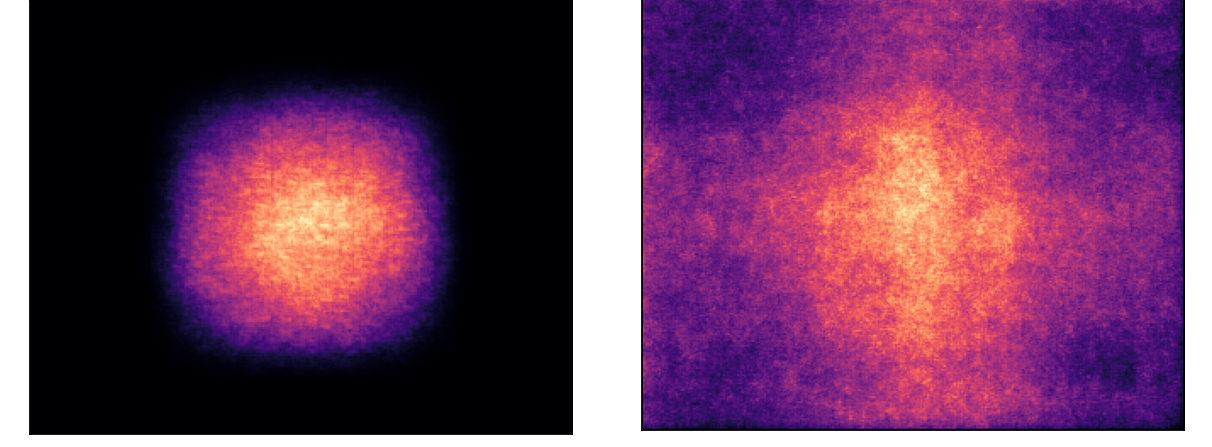
\includegraphics[width=\textwidth]{figs/erf_stage3_notitle.png}
  \caption{\textbf{How much of the frame each model uses} (stage 3, trained weights). Left: ResNet-18 in
  EventSSM, spread $\sigma=41.8$\,px. Right: BiMamba in PureSSM, $\sigma=85.6$\,px. At stage 4 the gap
  persists ($84.4$ vs $105.5$\,px).}
  \label{fig:erf}
\end{subfigure}\hfill
\begin{subfigure}[t]{0.40\textwidth}
  \centering
  \includegraphics[width=\textwidth]{figs/truerate_curve.pdf}
  \caption{\textbf{Accuracy when the event rate really changes.} Solid $=$ uncorrected, dashed $=$ with the
  published correction. The correction makes every model \emph{worse}.}
  \label{fig:rate}
\end{subfigure}
\end{figure}

\textbf{(a) The large-object win has a visible cause, and the reach is \emph{learned}}
(Fig.~\ref{fig:erf}). The SSM sees wider at every depth: a large object outside the convolution's reach
falls inside the SSM's. More interesting: training \emph{widened} the SSM's reach by ${\sim}30$\,px while
leaving the convolution's fixed. A scan can be taught to use long-range context; a convolution stack's reach
is fixed by its architecture. This turns the large-object number from an observation into an explanation.

\textbf{(b) The robustness is effective} (Fig.~\ref{fig:rate}).
When the event rate is changed by $10\times$, PureSSM keeps $69.7\%$ of its accuracy, the best of
everything tested (EventSSM $63.0\%$, S5-RVT $62.2\%$, the literature's ConvLSTM detector $17.7\%$). Since
EventSSM and PureSSM share an identical temporal path, the extra robustness must come from the spatial scan,
the same wide-reach advantage paying off again. However, the inference-time correction the original
paper credits for this robustness failed at all 19 evaluations (at true
$10\times$ it \emph{costs} ${\sim}13$\,mAP), and its headline 200\,Hz figure could not be reproduced from its
own checkpoint and code.

%%%%%%%%%%%%%%%%%%%%%%%%%%%%%%%%%%%%%%%%%%%%%%%%%%%%%%%%%%%%%%%
\section{Label quality: the models find objects the dataset never labelled}

\begin{figure}[htbp]
\centering
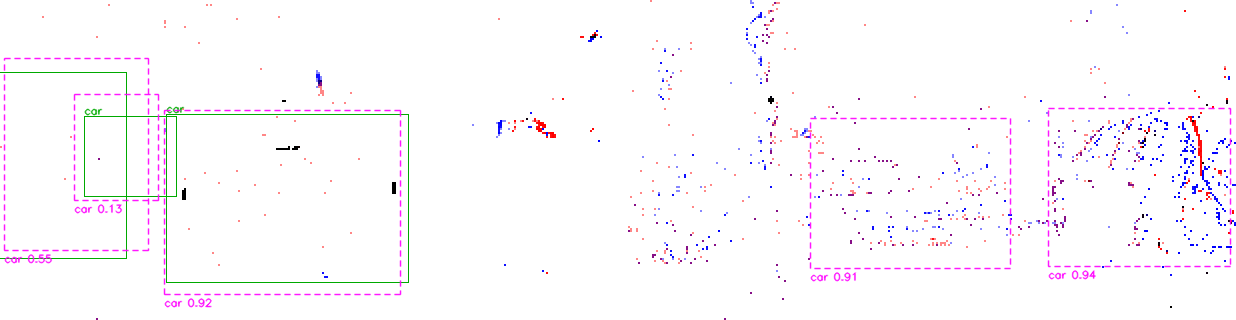
\includegraphics[width=0.92\textwidth]{figs/label_noise.png}
\caption{PureSSM on Gen1 test. \textcolor{green}{Green} $=$ dataset ground truth,
\textcolor{magenta}{magenta dashed} $=$ model prediction. \textbf{Left} ($t=25.7$\,s): the model matches the
labelled cars \emph{and} flags two more vehicles that carry no label. \textbf{Right} ($t=51.4$\,s): two
confident detections (0.91, 0.94) where the dataset gives no boxes at all. Each is scored as a mistake.}
\label{fig:labels}
\end{figure}

Gen1's boxes are incomplete: labels exist at only ${\sim}0.9$\,Hz, and
even within labelled frames clearly visible vehicles carry no box. Both models routinely produce confident,
correctly placed detections for objects the dataset never annotated (Fig.~\ref{fig:labels}), and the
evaluator counts every one as a false positive. All reported mAP figures therefore understate real detection
ability, for all three models alike. One test recording carries 117 car boxes to 11
pedestrian, which is also why pedestrian accuracy is low (${\sim}31$) for \emph{every} model. Since all
models are scored against the same imperfect key the comparison stays fair; what this caps is the ceiling,
not the ranking.

%%%%%%%%%%%%%%%%%%%%%%%%%%%%%%%%%%%%%%%%%%%%%%%%%%%%%%%%%%%%%%%
\section{Efficiency: a trade-off, not a free win}

\begin{table}[!htbp]
\centering\small
\setlength{\tabcolsep}{5pt}
\begin{tabularx}{\textwidth}{@{}Y C C C@{}}
\toprule
\textbf{Streaming inference}, RTX 5070 Ti & \textbf{S5-RVT} & \textbf{EventSSM} & \textbf{PureSSM} \\
\midrule
FLOPs per frame (G) & 11.89 & 13.55 & \textbf{10.12} \\
\textbf{Accuracy per GFLOP} & 4.01 & 3.41 & \textbf{4.59} \\
\addlinespace[1pt]
Speed, standard (Hz) & 58 & \textbf{79} & 37 \\
Speed, deploy mode (Hz) & not captured & \textbf{210} & 181 \\
\addlinespace[1pt]
Energy (J per frame) & 0.723 & \textbf{0.438} & 0.652 \\
Memory per camera stream & \textbf{4.7\,MB} & 144\,MB & 144\,MB \\
\bottomrule
\end{tabularx}
\end{table}

PureSSM does the least work (fewest FLOPs and parameters) and gets the most accuracy per unit
of work, yet is \emph{slowest} on the clock in standard mode. Its backbone is many small scan operations, so
the GPU spends more time starting work than doing it; an optimised deployment mode recovers most of it
($37 \rightarrow 181$\,Hz, comfortably real-time), though in the same mode EventSSM stays ahead. Two results
cut the other way: event sparsity buys no GPU speed-up, and the SSM's state makes the memory held per
stream $31\times$ larger than the baseline's, which matters most for a power-limited drone.

%%%%%%%%%%%%%%%%%%%%%%%%%%%%%%%%%%%%%%%%%%%%%%%%%%%%%%%%%%%%%%%
\section{Proposed Thesis C: spiking state-space models on Intel Loihi 2}

That last point motivates the next phase. Event sparsity is wasted on a GPU because dense kernels process idle
pixels anyway; on neuromorphic hardware they cost no energy, so the sparsity this thesis could not exploit
becomes a direct advantage. The proposal is to build and benchmark a spiking state-space detector on
Intel's Loihi 2.

\begin{itemize}[leftmargin=1.3em, itemsep=0pt, topsep=1pt]
  \item \textbf{Why it should work.} The temporal core is a diagonal linear recurrence of independent scalar
  states that map directly onto Loihi 2's per-neuron dynamics. Published work has mapped this model class to
  Loihi 2 at ${\sim}1000\times$ lower energy than a Jetson Orin Nano.
  \item \textbf{The obstacle, up front.} Mamba's input-dependent time step does not map cleanly to fixed
  neuron hardware. Staged plan: a fixed-step spiking model first (proven mappable), then push toward
  input-dependent behaviour on chip.
\end{itemize}

\textbf{A second option, lower priority.} Both models above are drop-in backbones inside the verified S5-RVT
pipeline, which is what keeps the comparison clean: neck, head, losses and evaluator are held fixed, so every
change traces to the backbone alone. The alternative is to write the full detector from scratch, including
the data pipeline, neck, head and loss, instead of inheriting parts designed around a convolutional recurrent
detector. That would let the architecture be shaped around state-space models end to end, at the cost of
direct comparability with published Gen1 numbers. Loihi remains the main
next step; this is the option to fall back on if hardware access stalls.

\end{document}
